\subsection{Opis hipotezy}\label{opis-hipotezy}

\textbf{Numer:} 8\\\textbf{Nazwa:} Liczba wypadków a
czas\\\textbf{Treść:} W ciągu dnia wypadków może być więcej w godzinach
szczytu, wieczorem w okolicach zmroku, kiedy widoczność jest najgorsza.
W ciągu roku mogłoby być ich więcej w zimie, z powodu gorszych warunków.
W skali roku na poziomie dni może ich być njawięcej w okolicach świąt,
gdyż jest wtedy wzmożony ruch i więcej pijanych kierowców (patrz
\href{Hipoteza-5}{hipoteza 5}).

\subsection{Wyniki związane z
hipotezą}\label{wyniki-zwiazane-z-hipoteza}

Dzień
tygodnia:\\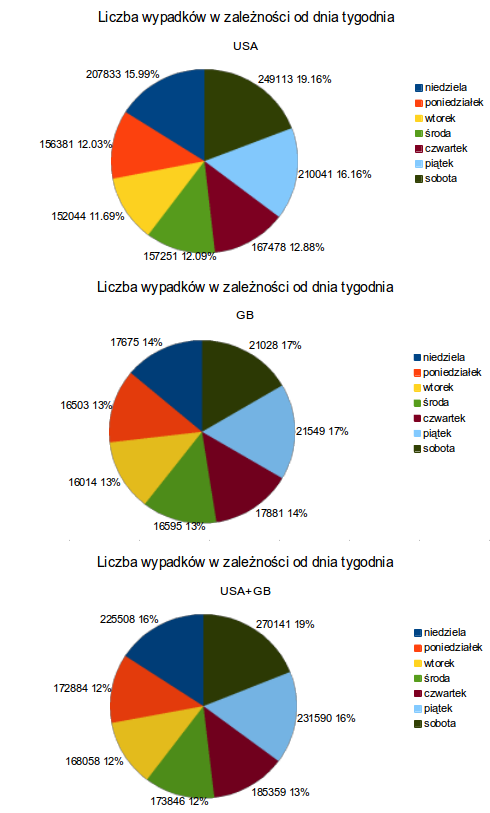
\includegraphics[width=0.8\textwidth]{images/statistics/day_of_week.png}

Rok:\\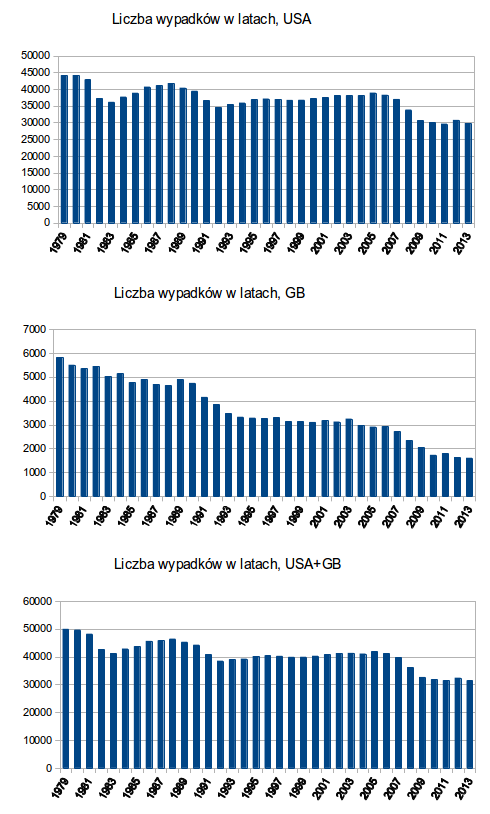
\includegraphics[width=0.8\textwidth]{images/statistics/year.png}

Miesiąc:\\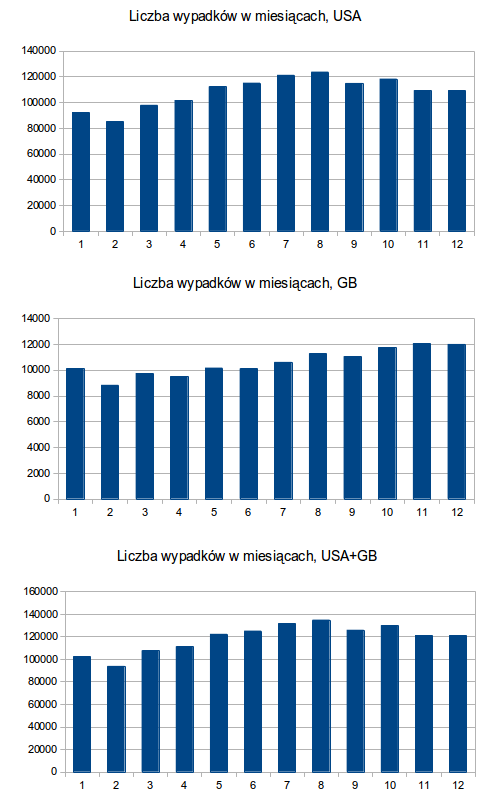
\includegraphics[width=0.8\textwidth]{images/statistics/month.png}

Dzień:\\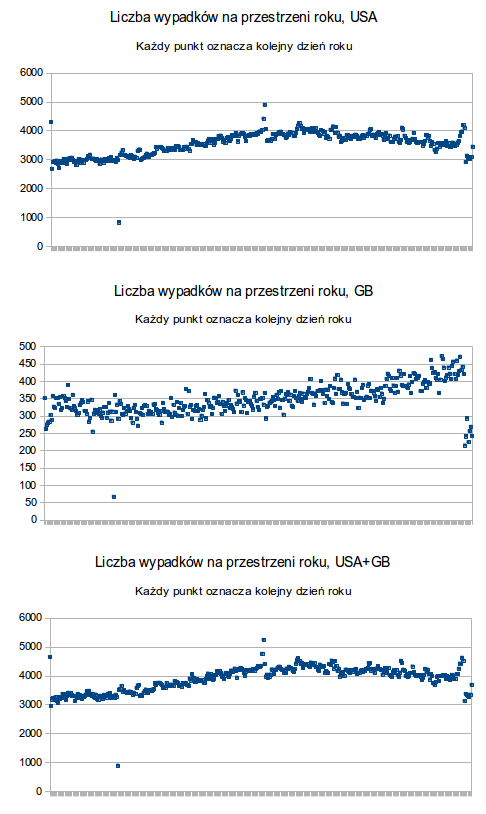
\includegraphics[width=0.8\textwidth]{images/statistics/day_of_year.png}

Bardzo niska wartość jest dla 29.02 - występuje tylko w latach
przestępnych i istotnie jest to wartość średnio 4 razy mniejsza.

Lokalne ``piki'' - \textbf{USA}:

\begin{itemize}
\itemsep1pt\parskip0pt\parsep0pt
\item
  01.01\\
\item
  03.07\\
\item
  04.07\\
\item
  02.08\\
\item
  03.08\\
\item
  31.10\\
\item
  01.11\\
\item
  20.12\\
\item
  21.12\\
\item
  22.12\\
\item
  23.12\\
\item
  24.12\\
\item
  31.12
\end{itemize}

Lokalne ``piki'' - \textbf{GB}:

\begin{itemize}
\itemsep1pt\parskip0pt\parsep0pt
\item
  21.01\\
\item
  01.03\\
\item
  18.04\\
\item
  01.05\\
\item
  15.08\\
\item
  07.09\\
\item
  20.10\\
\item
  30.10\\
\item
  05.12\\
\item
  21.12
\end{itemize}

Ciekawy jest spadek liczby wypadków w ostatnich dniach roku -
spowodowany prawdopodobnie faktem, że w tym okresie znacznie mniej osób
jeździ do pracy i spędza więcej czasu w domu z rodziną.

Godzina:\\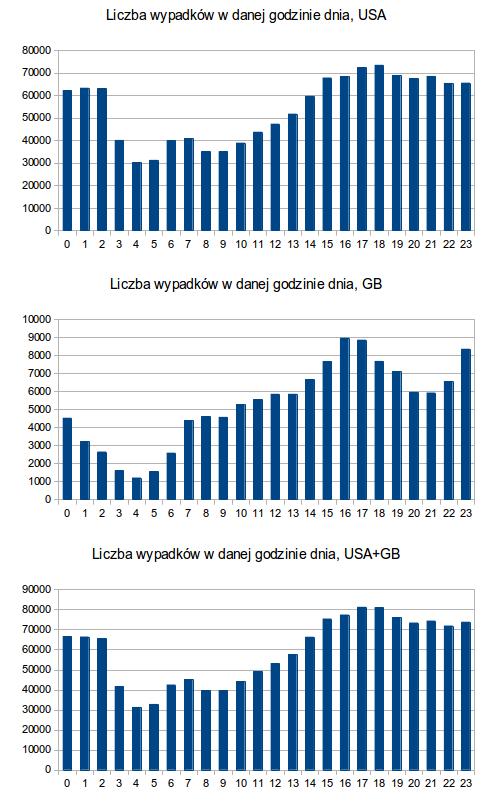
\includegraphics[width=0.8\textwidth]{images/statistics/hour.png}

\subsection{Weryfikacja i wnioski}\label{weryfikacja-i-wnioski}

Hipoteza analityczna dotycząca liczby wypadków w czasie w znacznej
mierze się potwierdziła. Podzielimy wyniki tej analizy w zależności od
rozważanych wymiarów czasowych

\subsubsection{Godzina}\label{godzina}

Bardzo wyraźnie widać wrost liczby wypadków w godzinach szczytu - w
trakcie powrotów z pracy. W Wielkiej Brytanii są to przede wszystkim
okolice godziny 16 i 17, w USA godzina 17-18. Widać również kiedy rano
ruch się zaczyna wzmagać i jest to w okolicach godziny 7, jednak nie ma
tak dużego skoku ilości wypadków dla porannej pory dojazdu do pracy.
Może to być związane z faktem że w drodze powrotnej kierowcy są bardziej
rozkojarzeni i zmęczeni niż rano. Porównanie Wielkiej Brytani i USA
pokazuje również, że w USA znacznie więcej wypadków zdarza się we
wczesnych godzinach nocnych (23 - 2). Powodem takiego stanu rzeczy może
być na przykład większy ruch tranzytowy w tych godzinach lub częstszy
wybór samochodu jako środka transportu w przypadku późnego powrotu do
domu.

\subsubsection{Miesiąc}\label{miesiac}

Analizując liczbę wypadków w kolejnych miesiącach widzimy znaczne
różnice między rozkładem w Wielkiej Brytanii i USA. W Stanach, wyraźne
nasilenie ilości wypadków jest w miesiącach wakacyjnych, mimo że można
się spodziewać, że warunki pogodowe będą wtedy lepsze. Nasilenie ruchu
musi byc znacznie większe w tym czasie, może być też większa brawura
kierowców. W Wielkiej Brytanii można bardziej wnioskować o korelacji
między warunkami pogodowymi a liczbą wypadków. Okazuje się że
najniebezpieczniejsze są październik, listopad i grudzień, kiedy warunki
nie są aż tak wymagające jak w styczniu czy w lutym, jednak ludzie nie
unikają jazdy samochodem i nie uważają tak bardzo jak w miesiącach
ściśle zimowych.

\subsubsection{Dzień tygodnia}\label{dzien-tygodnia}

Potwierdziła się hipoteza o większej liczbie wypadków w weekend. Jeżeli
dodamy wartości liczby wypadków dla piątku, soboty i niedzieli, zarówno
dla Wielkiej Brytanii jak i dla USA stanowią one około połowy całkowitej
liczby wypadków.

\subsubsection{Dzień}\label{dzien}

Z analizy rozkładu liczby wypadków na dni w ciągu roku można
zidentyfikować niektóre dni wolne. W USA wybija się 4 lipca - dzień
niepodległości. Można zauważyć wzrost np przed Halloween czy przed 6.12.
Wzrost można obserwować w okolicach Obserwujemy spadek liczby wypadków w
okresie świątecznym, kiedy ludzie mają wolne w pracy i przeważnie
spędzają ten czas w domu z rodziną.
